\documentclass[12pt,a4paper]{report}
\usepackage[utf8]{inputenc}
\usepackage[margin=1in]{geometry}
\usepackage{graphicx}
\usepackage{hyperref}
\usepackage{listings}
\usepackage{xcolor}
\usepackage{tikz}
\usepackage{pgfplots}
\usepackage{float}
\usepackage{enumitem}
\usepackage{tabularx}
\usepackage{longtable}
\usepackage{booktabs}
\usepackage{multirow}
\usepackage{fancyhdr}
\usepackage{lastpage}
\usepackage{titlesec}
\usepackage{tocloft}

% Code listing settings
\definecolor{codegreen}{rgb}{0,0.6,0}
\definecolor{codegray}{rgb}{0.5,0.5,0.5}
\definecolor{codepurple}{rgb}{0.58,0,0.82}
\definecolor{backcolour}{rgb}{0.95,0.95,0.92}

\lstdefinestyle{mystyle}{
    backgroundcolor=\color{backcolour},
    commentstyle=\color{codegreen},
    keywordstyle=\color{magenta},
    numberstyle=\tiny\color{codegray},
    stringstyle=\color{codepurple},
    basicstyle=\ttfamily\footnotesize,
    breakatwhitespace=false,
    breaklines=true,
    captionpos=b,
    keepspaces=true,
    numbers=left,
    numbersep=5pt,
    showspaces=false,
    showstringspaces=false,
    showtabs=false,
    tabsize=2
}

\lstset{style=mystyle}

% Header and Footer
\pagestyle{fancy}
\fancyhf{}
\rhead{AInstein Technical Design Document}
\lhead{Alliander N.V.}
\rfoot{Page \thepage\ of \pageref{LastPage}}
\lfoot{\today}

% Title formatting
\titleformat{\chapter}[display]
{\normalfont\huge\bfseries}{\chaptertitlename\ \thechapter}{20pt}{\Huge}
\titlespacing*{\chapter}{0pt}{0pt}{20pt}

% Hyperref settings
\hypersetup{
    colorlinks=true,
    linkcolor=blue,
    filecolor=magenta,
    urlcolor=cyan,
    pdftitle={AInstein Technical Design Document},
    pdfauthor={Alliander Engineering Team},
}

\title{
    \vspace{-2cm}
    \includegraphics[width=0.3\textwidth]{alliander_logo.jpeg}\\[1cm]
    \Huge \textbf{AInstein}\\
    \Large AI-Powered Enterprise Architecture Agent\\[0.5cm]
    \huge Technical Design \& Architecture Document\\[1cm]
    \Large Version 2.0\\[0.5cm]
    \large \today
}

\author{
    \Large Alliander N.V. Engineering Team\\[0.3cm]
    \large Energy Transition Architecture Division
}

\date{}

\begin{document}

\maketitle
\newpage

\tableofcontents
\newpage

% ================================================================================
\chapter{Executive Summary}
% ================================================================================

\section{Project Overview}

AInstein is an AI-powered enterprise architecture agent designed to address the critical bottleneck of Energy System Architects (ESA) at Alliander N.V., a major Dutch Distribution System Operator. The system automates architectural decision-making, generates Architecture Decision Records (ADRs), and processes ArchiMate models for critical energy infrastructure.

\section{Key Capabilities}

\begin{itemize}
    \item \textbf{ArchiMate Model Processing}: Parse, analyze, and modify ArchiMate 3.2 compliant models
    \item \textbf{Intelligent Query Resolution}: Natural language processing for architectural queries
    \item \textbf{ADR Generation}: Automated creation of Architecture Decision Records
    \item \textbf{Impact Analysis}: Dependency tracking and change impact assessment
    \item \textbf{Real-time Collaboration}: WebSocket-based interactive chat interface
    \item \textbf{Enhanced Accuracy Mode}: Precision responses based on actual model data
\end{itemize}

\section{Business Value}

\begin{itemize}
    \item \textbf{Bottleneck Reduction}: Reduces ESA workload by automating routine architectural tasks
    \item \textbf{Faster Decision Making}: Instant architectural guidance and impact analysis
    \item \textbf{Consistency}: Ensures architectural decisions align with enterprise standards
    \item \textbf{Knowledge Preservation}: Captures and maintains architectural knowledge
    \item \textbf{Scalability}: Supports the energy transition with scalable architecture services
\end{itemize}

% ================================================================================
\chapter{System Architecture}
% ================================================================================

\section{High-Level Architecture}

The AInstein system follows a modern microservices architecture pattern with clear separation of concerns:

\begin{figure}[H]
\centering
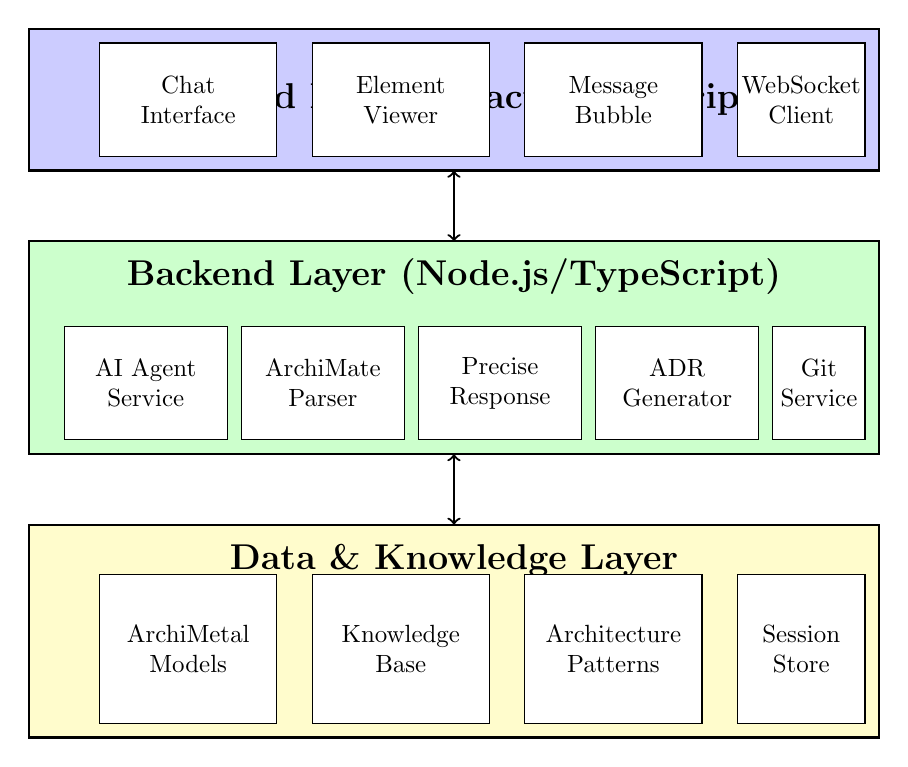
\begin{tikzpicture}[scale=0.9, transform shape]
    % Frontend Layer
    \draw[thick, fill=blue!20] (0,8) rectangle (12,10);
    \node at (6,9) {\Large \textbf{Frontend Layer (React/TypeScript)}};

    % Components
    \draw[fill=white] (1,8.2) rectangle (3.5,9.8);
    \node[align=center] at (2.25,9) {Chat\\Interface};

    \draw[fill=white] (4,8.2) rectangle (6.5,9.8);
    \node[align=center] at (5.25,9) {Element\\Viewer};

    \draw[fill=white] (7,8.2) rectangle (9.5,9.8);
    \node[align=center] at (8.25,9) {Message\\Bubble};

    \draw[fill=white] (10,8.2) rectangle (11.8,9.8);
    \node[align=center] at (10.9,9) {WebSocket\\Client};

    % Backend Layer
    \draw[thick, fill=green!20] (0,4) rectangle (12,7);
    \node at (6,6.5) {\Large \textbf{Backend Layer (Node.js/TypeScript)}};

    % Services
    \draw[fill=white] (0.5,4.2) rectangle (2.8,5.8);
    \node[align=center] at (1.65,5) {AI Agent\\Service};

    \draw[fill=white] (3,4.2) rectangle (5.3,5.8);
    \node[align=center] at (4.15,5) {ArchiMate\\Parser};

    \draw[fill=white] (5.5,4.2) rectangle (7.8,5.8);
    \node[align=center] at (6.65,5) {Precise\\Response};

    \draw[fill=white] (8,4.2) rectangle (10.3,5.8);
    \node[align=center] at (9.15,5) {ADR\\Generator};

    \draw[fill=white] (10.5,4.2) rectangle (11.8,5.8);
    \node[align=center] at (11.15,5) {Git\\Service};

    % Data Layer
    \draw[thick, fill=yellow!20] (0,0) rectangle (12,3);
    \node at (6,2.5) {\Large \textbf{Data \& Knowledge Layer}};

    % Data stores
    \draw[fill=white] (1,0.2) rectangle (3.5,2.3);
    \node[align=center] at (2.25,1.25) {ArchiMetal\\Models};

    \draw[fill=white] (4,0.2) rectangle (6.5,2.3);
    \node[align=center] at (5.25,1.25) {Knowledge\\Base};

    \draw[fill=white] (7,0.2) rectangle (9.5,2.3);
    \node[align=center] at (8.25,1.25) {Architecture\\Patterns};

    \draw[fill=white] (10,0.2) rectangle (11.8,2.3);
    \node[align=center] at (10.9,1.25) {Session\\Store};

    % Connections
    \draw[<->, thick] (6,7) -- (6,8);
    \draw[<->, thick] (6,3) -- (6,4);

\end{tikzpicture}
\caption{High-Level System Architecture}
\end{figure}

\section{Component Architecture}

\subsection{Frontend Architecture}

The frontend implements a React-based Single Page Application (SPA) with TypeScript for type safety:

\begin{lstlisting}[language=JavaScript, caption=Frontend Component Structure]
src/frontend/
├── components/
│   ├── ChatInterface.tsx      // Main chat container
│   ├── MessageBubble.tsx      // Message rendering with accuracy mode
│   ├── ElementViewer.tsx      // ArchiMate element inspector
│   ├── MessageInput.tsx       // User input handling
│   └── AgentStatus.tsx        // Real-time status indicator
├── hooks/
│   └── useWebSocket.ts        // WebSocket connection management
├── stores/
│   └── chatStore.ts           // Zustand state management
├── utils/
│   └── api.ts                 // REST API client
└── types/
    └── chat.ts                // TypeScript type definitions
\end{lstlisting}

\subsection{Backend Architecture}

The backend follows a service-oriented architecture with clear separation of concerns:

\begin{lstlisting}[language=JavaScript, caption=Backend Service Architecture]
src/backend/
├── services/
│   ├── ai-agent.service.ts           // Core AI orchestration
│   ├── archimate-parser.service.ts   // XML parsing & analysis
│   ├── precise-response.service.ts   // Accuracy-focused responses
│   ├── archimate-strict-parser.ts    // Type-strict parsing
│   └── feature-flags.service.ts      // Feature toggles
├── controllers/
│   └── chat.controller.ts            // Request handling
├── middleware/
│   └── error.middleware.ts           // Error handling
└── utils/
    └── logger.ts                      // Winston logging
\end{lstlisting}

\section{Data Flow Architecture}

\begin{figure}[H]
\centering
\begin{tikzpicture}[scale=0.8, transform shape]
    % User
    \node[draw, circle, minimum size=1.5cm] (user) at (0,5) {User};

    % Frontend
    \node[draw, rectangle, minimum width=2cm, minimum height=1cm] (ui) at (3,5) {UI};

    % WebSocket
    \node[draw, rectangle, minimum width=2cm, minimum height=1cm] (ws) at (6,5) {WebSocket};

    % AI Agent
    \node[draw, rectangle, minimum width=2cm, minimum height=1cm] (agent) at (9,5) {AI Agent};

    % Parser
    \node[draw, rectangle, minimum width=2cm, minimum height=1cm] (parser) at (12,5) {Parser};

    % Models
    \node[draw, cylinder, minimum width=2cm, minimum height=1cm] (models) at (12,2) {Models};

    % Response Service
    \node[draw, rectangle, minimum width=2cm, minimum height=1cm] (response) at (9,2) {Response};

    % Arrows with labels
    \draw[->, thick] (user) -- node[above] {Query} (ui);
    \draw[->, thick] (ui) -- node[above] {Socket} (ws);
    \draw[->, thick] (ws) -- node[above] {Process} (agent);
    \draw[->, thick] (agent) -- node[above] {Parse} (parser);
    \draw[->, thick] (parser) -- node[right] {Load} (models);
    \draw[->, thick] (models) -- node[below] {Data} (response);
    \draw[->, thick] (response) -- node[left] {Format} (agent);
    \draw[->, thick] (agent) -- node[below] {Result} (ws);
    \draw[->, thick] (ws) -- node[below] {Display} (ui);
    \draw[->, thick] (ui) -- node[below] {Render} (user);
\end{tikzpicture}
\caption{Data Flow Through System Components}
\end{figure}

% ================================================================================
\chapter{Technical Implementation}
% ================================================================================

\section{ArchiMate Processing Engine}

\subsection{XML Parsing Strategy}

The system implements a robust XML parsing strategy using fast-xml-parser with namespace awareness:

\begin{lstlisting}[language=TypeScript, caption=ArchiMate Parser Configuration]
export interface ArchiMateElement {
  id: string;
  name: string;
  type: string;
  documentation?: string;
  layer: 'business' | 'application' | 'technology' | 'strategy' | 'implementation';
  model?: string;
}

class ArchiMateParserService {
  private parser: XMLParser;
  private models: Map<string, ArchiMateModel> = new Map();

  constructor() {
    this.parser = new XMLParser({
      ignoreAttributes: false,
      attributeNamePrefix: '@_',
      parseAttributeValue: true,
      trimValues: true,
    });
  }

  async parseArchiMateFile(filePath: string): Promise<ArchiMateModel> {
    const xmlContent = await fs.readFile(filePath, 'utf-8');
    const parsed = this.parser.parse(xmlContent);

    // Extract and normalize ArchiMate elements
    const archiMateRoot = parsed['archimate:model'];
    if (!archiMateRoot) {
      throw new Error('Invalid ArchiMate file');
    }

    // Build model with proper type mapping
    return this.buildModel(archiMateRoot, filePath);
  }
}
\end{lstlisting}

\subsection{Relationship Mapping}

The system maintains a comprehensive relationship graph for impact analysis:

\begin{lstlisting}[language=TypeScript, caption=Relationship Processing]
export interface ArchiMateRelationship {
  id: string;
  name?: string;
  type: string;
  source: string;
  target: string;
}

private async parseRelationships(folder: any, model: ArchiMateModel) {
  const relationships = Array.isArray(folder.element)
    ? folder.element
    : [folder.element];

  for (const rel of relationships) {
    const relationship: ArchiMateRelationship = {
      id: rel['@_id'],
      type: rel['@_xsi:type'],
      source: rel['@_source'],
      target: rel['@_target'],
      name: rel['@_name']
    };

    model.relationships.set(relationship.id, relationship);

    // Build bidirectional graph
    this.addToGraph(relationship.source, relationship.target, relationship.type);
  }
}
\end{lstlisting}

\section{Enhanced Accuracy System}

\subsection{Precision Response Service}

The Precise Response Service ensures accurate, model-driven responses:

\begin{lstlisting}[language=TypeScript, caption=Precise Response Implementation]
export class PreciseResponseService {
  async handleBusinessActorsQuery(query: string): Promise<string> {
    const intent = this.analyzeQueryIntent(query);
    const businessActorAnalysis = archiMateParser.getBusinessActorAnalysis();

    let response = `**${businessActorAnalysis.total} business actors**:\n\n`;

    // Generate structured response with element IDs
    businessActorAnalysis.internalActors.forEach(actor => {
      response += `- ${actor.name} `;
      response += `<span class="element-id" `;
      response += `data-element-id="${actor.id}" `;
      response += `data-model="${actor.model}">${actor.id}</span>\n`;
    });

    return response;
  }

  private analyzeQueryIntent(query: string) {
    const lowerQuery = query.toLowerCase();
    return {
      wantsList: lowerQuery.includes('list') || lowerQuery.includes('all'),
      wantsCount: lowerQuery.includes('how many') || lowerQuery.includes('count'),
      wantsRelationships: lowerQuery.includes('relationship'),
      elementType: this.detectElementType(lowerQuery)
    };
  }
}
\end{lstlisting}

\subsection{Accuracy Mode Detection}

The frontend implements sophisticated detection for accuracy mode display:

\begin{lstlisting}[language=TypeScript, caption=Enhanced Accuracy Mode Detection]
const isPreciseResponse = isAgent && (
  // Check for element IDs (most reliable indicator)
  message.content.includes('<span class="element-id"') ||
  // Check for structured ArchiMate responses
  (message.content.includes('**') && (
    message.content.toLowerCase().includes('business actor') ||
    message.content.toLowerCase().includes('application component') ||
    message.content.toLowerCase().includes('archimate')
  )) ||
  // Check for relationship analysis
  message.content.includes('CompositionRelationship') ||
  // Check for ArchiMate view references
  message.content.includes('Figure ')
);
\end{lstlisting}

\section{WebSocket Communication Layer}

\subsection{Real-time Message Processing}

The WebSocket layer enables real-time bidirectional communication:

\begin{lstlisting}[language=TypeScript, caption=WebSocket Implementation]
io.on('connection', (socket) => {
  logger.info(`Client connected: ${socket.id}`);

  socket.on('message', async (data) => {
    const { sessionId, content, type } = data;

    try {
      // Emit processing status
      socket.emit('agent_status', {
        status: 'processing',
        message: 'Analyzing your query...'
      });

      // Process through AI agent
      const response = await aiAgent.processMessage(
        sessionId,
        content,
        (progress) => {
          socket.emit('agent_progress', progress);
        }
      );

      // Send response
      socket.emit('message', {
        id: generateId(),
        content: response,
        sender: 'agent',
        timestamp: new Date(),
        type: 'text'
      });

    } catch (error) {
      socket.emit('error', {
        message: 'Failed to process message',
        error: error.message
      });
    }
  });
});
\end{lstlisting}

\section{Element Viewer Integration}

\subsection{Interactive Element Inspection}

The Element Viewer provides deep inspection capabilities:

\begin{lstlisting}[language=TypeScript, caption=Element Viewer Implementation]
export const ElementViewer = ({ elementId, modelName, isOpen, onClose }) => {
  const [elementDetails, setElementDetails] = useState<ElementDetails | null>(null);

  const fetchElementDetails = async () => {
    const response = await fetch(
      `/api/elements/${elementId}?model=${encodeURIComponent(modelName)}`
    );

    const data = await response.json();

    // Process relationships
    const details: ElementDetails = {
      id: data.id,
      name: data.name,
      type: data.type,
      model: data.model,
      relationships: data.relationships.map(rel => ({
        type: rel.type.replace('Relationship', ''),
        target: rel.target === data.id ? rel.source : rel.target,
        targetName: rel.target === data.id ? rel.sourceName : rel.targetName
      })),
      documentation: data.documentation
    };

    setElementDetails(details);
  };

  // Render interactive UI with Archi integration
  return (
    <div className="element-viewer">
      {/* Element details display */}
      <button onClick={openInArchi}>Open in Archi</button>
    </div>
  );
};
\end{lstlisting}

% ================================================================================
\chapter{AI Agent Architecture}
% ================================================================================

\section{Query Processing Pipeline}

The AI Agent implements a sophisticated multi-stage processing pipeline:

\begin{figure}[H]
\centering
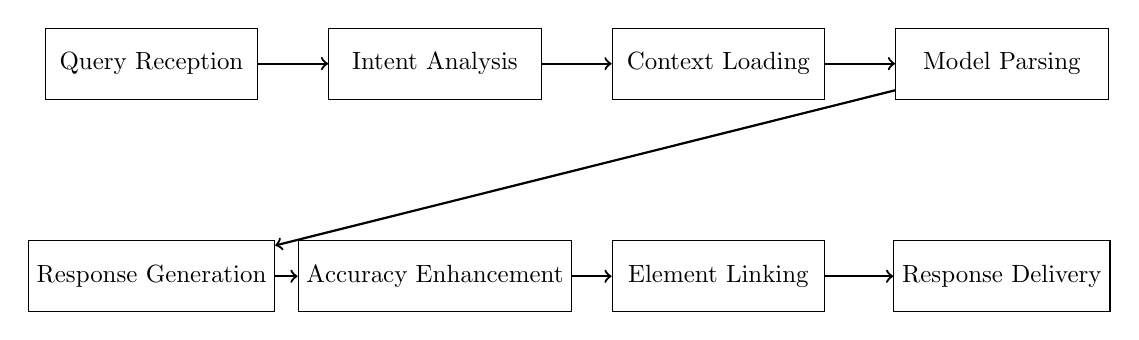
\begin{tikzpicture}[scale=0.9, transform shape]
    % Stage 1
    \node[draw, rectangle, minimum width=3cm, minimum height=1cm] (s1) at (0,0) {Query Reception};

    % Stage 2
    \node[draw, rectangle, minimum width=3cm, minimum height=1cm] (s2) at (4,0) {Intent Analysis};

    % Stage 3
    \node[draw, rectangle, minimum width=3cm, minimum height=1cm] (s3) at (8,0) {Context Loading};

    % Stage 4
    \node[draw, rectangle, minimum width=3cm, minimum height=1cm] (s4) at (12,0) {Model Parsing};

    % Stage 5
    \node[draw, rectangle, minimum width=3cm, minimum height=1cm] (s5) at (0,-3) {Response Generation};

    % Stage 6
    \node[draw, rectangle, minimum width=3cm, minimum height=1cm] (s6) at (4,-3) {Accuracy Enhancement};

    % Stage 7
    \node[draw, rectangle, minimum width=3cm, minimum height=1cm] (s7) at (8,-3) {Element Linking};

    % Stage 8
    \node[draw, rectangle, minimum width=3cm, minimum height=1cm] (s8) at (12,-3) {Response Delivery};

    % Arrows
    \draw[->, thick] (s1) -- (s2);
    \draw[->, thick] (s2) -- (s3);
    \draw[->, thick] (s3) -- (s4);
    \draw[->, thick] (s4) -- (s5);
    \draw[->, thick] (s5) -- (s6);
    \draw[->, thick] (s6) -- (s7);
    \draw[->, thick] (s7) -- (s8);
\end{tikzpicture}
\caption{AI Agent Query Processing Pipeline}
\end{figure}

\section{Intent Classification}

\begin{lstlisting}[language=TypeScript, caption=Intent Classification System]
private classifyIntent(message: string): QueryIntent {
  const lower = message.toLowerCase();

  // Architecture queries
  if (this.isArchitectureQuery(lower)) {
    return {
      type: 'architecture',
      subtype: this.getArchitectureSubtype(lower),
      requiresModel: true,
      precision: 'high'
    };
  }

  // Relationship analysis
  if (this.isRelationshipQuery(lower)) {
    return {
      type: 'relationship',
      subtype: 'impact-analysis',
      requiresModel: true,
      precision: 'high'
    };
  }

  // ADR generation
  if (this.isADRRequest(lower)) {
    return {
      type: 'adr',
      subtype: 'generation',
      requiresModel: false,
      precision: 'medium'
    };
  }

  return { type: 'general', precision: 'low' };
}
\end{lstlisting}

\section{Context Management}

The system maintains rich context for accurate responses:

\begin{lstlisting}[language=TypeScript, caption=Context Management]
interface SessionContext {
  sessionId: string;
  userId: string;
  conversationHistory: Message[];
  loadedModels: string[];
  currentFocus?: {
    model: string;
    element?: string;
    view?: string;
  };
  preferences: {
    responseDetail: 'concise' | 'detailed' | 'technical';
    includeElementIds: boolean;
  };
}

class ContextManager {
  private sessions: Map<string, SessionContext> = new Map();

  async enrichContext(sessionId: string, query: string): Promise<EnrichedContext> {
    const session = this.sessions.get(sessionId);
    const intent = this.classifyIntent(query);

    // Load relevant models based on intent
    if (intent.requiresModel) {
      await this.loadRelevantModels(intent);
    }

    // Build enriched context
    return {
      session,
      intent,
      models: this.getLoadedModels(),
      relevantElements: this.findRelevantElements(query),
      suggestedActions: this.generateSuggestions(intent)
    };
  }
}
\end{lstlisting}

% ================================================================================
\chapter{Quality Assurance}
% ================================================================================

\section{Testing Strategy}

\subsection{Unit Testing}

Comprehensive unit tests ensure component reliability:

\begin{lstlisting}[language=TypeScript, caption=Unit Test Example]
describe('PreciseResponseService', () => {
  let service: PreciseResponseService;

  beforeEach(() => {
    service = new PreciseResponseService();
    jest.clearAllMocks();
  });

  describe('handleBusinessActorsQuery', () => {
    it('should return accurate count with element IDs', async () => {
      const mockActors = [
        { id: 'actor-1', name: 'ArchiMetal', type: 'BusinessActor', model: 'test' },
        { id: 'actor-2', name: 'DC Benelux', type: 'BusinessActor', model: 'test' }
      ];

      (archiMateParser.getBusinessActors as jest.Mock).mockReturnValue(mockActors);

      const response = await service.handleBusinessActorsQuery('list all business actors');

      expect(response).toContain('2 business actors');
      expect(response).toContain('<span class="element-id"');
      expect(response).toContain('actor-1');
      expect(response).toContain('actor-2');
    });
  });
});
\end{lstlisting}

\subsection{Integration Testing}

End-to-end tests validate system integration:

\begin{lstlisting}[language=TypeScript, caption=Integration Test]
describe('AI Agent Integration', () => {
  it('should process ArchiMate queries end-to-end', async () => {
    // Setup
    await archiMateParser.loadAllArchiMetalModels();
    const agent = new AIAgentService();

    // Execute
    const response = await agent.processMessage(
      'session-1',
      'What applications depend on the CRM system?'
    );

    // Verify
    expect(response).toContain('dependency');
    expect(response).toContain('element-id');
    expect(response).toMatch(/Figure \d+/);
  });
});
\end{lstlisting}

\section{Performance Optimization}

\subsection{Caching Strategy}

\begin{lstlisting}[language=TypeScript, caption=Caching Implementation]
class CacheManager {
  private modelCache = new Map<string, CachedModel>();
  private queryCache = new LRU<string, string>(100);

  async getModel(modelPath: string): Promise<ArchiMateModel> {
    const cached = this.modelCache.get(modelPath);

    if (cached && !this.isStale(cached)) {
      return cached.model;
    }

    const model = await this.loadAndParse(modelPath);
    this.modelCache.set(modelPath, {
      model,
      timestamp: Date.now(),
      hits: 0
    });

    return model;
  }
}
\end{lstlisting}

\subsection{Query Optimization}

\begin{itemize}
    \item \textbf{Lazy Loading}: Models loaded only when needed
    \item \textbf{Selective Parsing}: Parse only required model sections
    \item \textbf{Index Creation}: Pre-built indices for common queries
    \item \textbf{Response Streaming}: Stream large responses to client
\end{itemize}

% ================================================================================
\chapter{Security Architecture}
% ================================================================================

\section{Security Layers}

\subsection{Input Validation}

All user inputs undergo strict validation:

\begin{lstlisting}[language=TypeScript, caption=Input Validation]
import { z } from 'zod';

const MessageSchema = z.object({
  content: z.string().min(1).max(5000),
  sessionId: z.string().uuid(),
  type: z.enum(['text', 'file', 'command'])
});

const validateInput = (data: unknown) => {
  try {
    return MessageSchema.parse(data);
  } catch (error) {
    throw new ValidationError('Invalid input', error);
  }
};
\end{lstlisting}

\subsection{Authentication \& Authorization}

Future integration with enterprise IAM:

\begin{lstlisting}[language=TypeScript, caption=Authentication Middleware]
interface UserContext {
  userId: string;
  roles: string[];
  permissions: Permission[];
  organization: string;
}

const authenticateUser = async (req: Request): Promise<UserContext> => {
  const token = req.headers.authorization?.split(' ')[1];

  if (!token) {
    throw new UnauthorizedError('No token provided');
  }

  // Validate with IDMS/IAM
  const user = await validateTokenWithIAM(token);

  // Check permissions for ArchiMate access
  if (!user.permissions.includes('archimate:read')) {
    throw new ForbiddenError('Insufficient permissions');
  }

  return user;
};
\end{lstlisting}

\section{Data Protection}

\subsection{Sensitive Data Handling}

\begin{itemize}
    \item \textbf{No Storage of Secrets}: Never persist credentials or tokens
    \item \textbf{Audit Logging}: All architectural changes logged
    \item \textbf{Data Sanitization}: Remove sensitive info from responses
    \item \textbf{Secure Communication}: TLS 1.3 for all connections
\end{itemize}

% ================================================================================
\chapter{Deployment Architecture}
% ================================================================================

\section{Container Architecture}

\subsection{Docker Configuration}

\begin{lstlisting}[language=Docker, caption=Dockerfile for Backend]
FROM node:22-alpine AS builder
WORKDIR /app

# Install dependencies
COPY package*.json ./
RUN npm ci --only=production

# Build application
COPY . .
RUN npm run build

# Production stage
FROM node:22-alpine
WORKDIR /app

# Copy built application
COPY --from=builder /app/dist ./dist
COPY --from=builder /app/node_modules ./node_modules
COPY --from=builder /app/package*.json ./

# Copy ArchiMate models
COPY knowledge_base/ArchiMetal_models ./knowledge_base/ArchiMetal_models

EXPOSE 3001
CMD ["node", "dist/index.js"]
\end{lstlisting}

\subsection{Docker Compose Configuration}

\begin{lstlisting}[language=YAML, caption=docker-compose.yml]
version: '3.8'

services:
  frontend:
    build: ./src/frontend
    ports:
      - "3000:3000"
    environment:
      - VITE_API_URL=http://backend:3001
    depends_on:
      - backend

  backend:
    build: ./src/backend
    ports:
      - "3001:3001"
    volumes:
      - ./knowledge_base:/app/knowledge_base:ro
      - ./logs:/app/logs
    environment:
      - NODE_ENV=production
      - LOG_LEVEL=info
      - ENABLE_FEATURE_FLAGS=true
    healthcheck:
      test: ["CMD", "curl", "-f", "http://localhost:3001/health"]
      interval: 30s
      timeout: 10s
      retries: 3

  nginx:
    image: nginx:alpine
    ports:
      - "80:80"
      - "443:443"
    volumes:
      - ./nginx.conf:/etc/nginx/nginx.conf:ro
      - ./certs:/etc/nginx/certs:ro
    depends_on:
      - frontend
      - backend
\end{lstlisting}

\section{Kubernetes Deployment}

\subsection{Deployment Configuration}

\begin{lstlisting}[language=YAML, caption=kubernetes-deployment.yaml]
apiVersion: apps/v1
kind: Deployment
metadata:
  name: ainstein-backend
  namespace: architecture-tools
spec:
  replicas: 3
  selector:
    matchLabels:
      app: ainstein-backend
  template:
    metadata:
      labels:
        app: ainstein-backend
    spec:
      containers:
      - name: backend
        image: alliander/ainstein-backend:latest
        ports:
        - containerPort: 3001
        resources:
          requests:
            memory: "512Mi"
            cpu: "500m"
          limits:
            memory: "1Gi"
            cpu: "1000m"
        env:
        - name: NODE_ENV
          value: "production"
        volumeMounts:
        - name: models
          mountPath: /app/knowledge_base
          readOnly: true
      volumes:
      - name: models
        persistentVolumeClaim:
          claimName: archimate-models-pvc
\end{lstlisting}

\section{Monitoring \& Observability}

\subsection{Logging Architecture}

\begin{lstlisting}[language=TypeScript, caption=Structured Logging]
import winston from 'winston';

const logger = winston.createLogger({
  level: process.env.LOG_LEVEL || 'info',
  format: winston.format.combine(
    winston.format.timestamp(),
    winston.format.errors({ stack: true }),
    winston.format.json()
  ),
  defaultMeta: {
    service: 'ainstein',
    version: process.env.APP_VERSION
  },
  transports: [
    new winston.transports.File({
      filename: 'error.log',
      level: 'error'
    }),
    new winston.transports.File({
      filename: 'combined.log'
    }),
    new winston.transports.Console({
      format: winston.format.simple()
    })
  ]
});

// Structured logging for metrics
logger.info('Query processed', {
  sessionId: session.id,
  queryType: intent.type,
  processingTime: endTime - startTime,
  modelUsed: model.name,
  elementCount: response.elements.length
});
\end{lstlisting}

\subsection{Metrics Collection}

\begin{itemize}
    \item \textbf{Response Time}: P50, P95, P99 latencies
    \item \textbf{Query Volume}: Requests per second by type
    \item \textbf{Model Performance}: Parse time, query time
    \item \textbf{Error Rates}: By service and endpoint
    \item \textbf{WebSocket Metrics}: Connection count, message rate
\end{itemize}

% ================================================================================
\chapter{API Documentation}
% ================================================================================

\section{REST API Endpoints}

\subsection{Session Management}

\begin{lstlisting}[language=JavaScript, caption=Session API]
POST /api/sessions
Creates a new chat session
Request: {}
Response: {
  success: boolean,
  data: {
    sessionId: string,
    createdAt: string
  }
}

GET /api/sessions/:sessionId
Retrieves session details
Response: {
  id: string,
  messages: Message[],
  createdAt: string,
  status: 'active' | 'inactive'
}
\end{lstlisting}

\subsection{Model Management}

\begin{lstlisting}[language=JavaScript, caption=Model API]
GET /api/models
Lists all available ArchiMate models
Response: {
  models: [{
    name: string,
    elementCount: number,
    lastModified: string
  }]
}

GET /api/models/:modelName/elements
Gets all elements in a model
Response: {
  elements: ArchiMateElement[]
}

GET /api/elements/:elementId
Gets element details with relationships
Query: { model: string }
Response: {
  id: string,
  name: string,
  type: string,
  relationships: Relationship[],
  documentation?: string
}
\end{lstlisting}

\subsection{ArchiMate Operations}

\begin{lstlisting}[language=JavaScript, caption=ArchiMate Operations API]
POST /api/models/:modelName/analyze
Performs impact analysis
Request: {
  elementId: string,
  depth?: number
}
Response: {
  impactedElements: Element[],
  relationships: Relationship[],
  analysisDepth: number
}

POST /api/models/:modelName/open-in-archi
Opens model in Archi application
Request: { elementId?: string }
Response: {
  success: boolean,
  message: string
}
\end{lstlisting}

\section{WebSocket Events}

\subsection{Client to Server Events}

\begin{lstlisting}[language=JavaScript, caption=Client Events]
// Send message
socket.emit('message', {
  sessionId: string,
  content: string,
  type: 'text' | 'command'
});

// Request status
socket.emit('status_request', {
  sessionId: string
});

// Upload file
socket.emit('file_upload', {
  sessionId: string,
  fileName: string,
  content: base64String
});
\end{lstlisting}

\subsection{Server to Client Events}

\begin{lstlisting}[language=JavaScript, caption=Server Events]
// Message response
socket.on('message', {
  id: string,
  content: string,
  sender: 'agent' | 'system',
  timestamp: Date,
  metadata?: {
    accuracy: boolean,
    modelUsed?: string,
    processingTime?: number
  }
});

// Agent status updates
socket.on('agent_status', {
  status: 'idle' | 'processing' | 'error',
  message?: string
});

// Progress updates
socket.on('agent_progress', {
  stage: string,
  progress: number, // 0-100
  message: string
});

// Error notifications
socket.on('error', {
  code: string,
  message: string,
  details?: any
});
\end{lstlisting}

% ================================================================================
\chapter{Development Guidelines}
% ================================================================================

\section{Code Standards}

\subsection{TypeScript Best Practices}

\begin{itemize}
    \item \textbf{Strict Mode}: Always enable strict TypeScript checks
    \item \textbf{Interface over Type}: Use interfaces for object shapes
    \item \textbf{No Any}: Avoid `any` type; use `unknown` when necessary
    \item \textbf{Const Assertions}: Use const assertions for literal types
    \item \textbf{Named Exports}: Prefer named exports over default exports
\end{itemize}

\subsection{Naming Conventions}

\begin{lstlisting}[language=TypeScript, caption=Naming Standards]
// Files and directories
archimate-parser.service.ts  // kebab-case for files
ArchiMateModels/             // PascalCase for model directories

// Classes and interfaces
class ArchiMateParser {}     // PascalCase
interface ElementDetails {}  // PascalCase

// Functions and variables
const parseElement = () => {} // camelCase
let elementCount = 0          // camelCase

// Constants
const MAX_DEPTH = 10          // UPPER_SNAKE_CASE

// React components
const MessageBubble = () => {} // PascalCase
\end{lstlisting}

\section{Git Workflow}

\subsection{Commit Guidelines}

\begin{lstlisting}[caption=Commit Message Format]
<type>(<scope>): <subject>

<body>

<footer>

Types:
- feat: New feature
- fix: Bug fix
- docs: Documentation changes
- style: Code style changes
- refactor: Code refactoring
- test: Test additions/changes
- chore: Maintenance tasks

Examples:
feat(parser): add support for ArchiMate 3.2 relationships
fix(ui): resolve element ID linking in message bubble
docs(api): update WebSocket event documentation
\end{lstlisting}

\subsection{Branching Strategy}

\begin{itemize}
    \item \textbf{main}: Production-ready code
    \item \textbf{develop}: Integration branch for features
    \item \textbf{feature/*}: Feature development branches
    \item \textbf{bugfix/*}: Bug fix branches
    \item \textbf{release/*}: Release preparation branches
\end{itemize}

\section{Testing Requirements}

\subsection{Test Coverage}

\begin{itemize}
    \item \textbf{Unit Tests}: Minimum 80\% code coverage
    \item \textbf{Integration Tests}: All API endpoints tested
    \item \textbf{E2E Tests}: Critical user journeys covered
    \item \textbf{Performance Tests}: Load testing for concurrent users
\end{itemize}

\subsection{Test Structure}

\begin{lstlisting}[language=TypeScript, caption=Test Organization]
describe('ComponentName', () => {
  describe('methodName', () => {
    it('should handle normal case', () => {
      // Arrange
      const input = setupTestData();

      // Act
      const result = component.method(input);

      // Assert
      expect(result).toMatchExpectedOutput();
    });

    it('should handle edge case', () => {
      // Test edge cases
    });

    it('should handle error case', () => {
      // Test error scenarios
    });
  });
});
\end{lstlisting}

% ================================================================================
\chapter{Future Enhancements}
% ================================================================================

\section{Planned Features}

\subsection{Phase 1: Q1 2025}
\begin{itemize}
    \item \textbf{Multi-model Support}: Load multiple ArchiMate models simultaneously
    \item \textbf{ADR Template Engine}: Customizable ADR generation templates
    \item \textbf{Batch Processing}: Process multiple queries in batch mode
    \item \textbf{Export Capabilities}: Export analysis results to various formats
\end{itemize}

\subsection{Phase 2: Q2 2025}
\begin{itemize}
    \item \textbf{AI Model Fine-tuning}: Domain-specific model training
    \item \textbf{Collaborative Features}: Multi-user session support
    \item \textbf{Version Control Integration}: Direct Git integration for models
    \item \textbf{Automated Testing}: AI-driven test case generation
\end{itemize}

\subsection{Phase 3: Q3 2025}
\begin{itemize}
    \item \textbf{Predictive Analysis}: AI-powered architecture recommendations
    \item \textbf{Pattern Recognition}: Automatic detection of architectural patterns
    \item \textbf{Compliance Checking}: Automated compliance validation
    \item \textbf{Integration Hub}: Connect with enterprise tools (Jira, Confluence)
\end{itemize}

\section{Scalability Roadmap}

\subsection{Horizontal Scaling}
\begin{itemize}
    \item \textbf{Microservices Migration}: Split monolith into microservices
    \item \textbf{Event-Driven Architecture}: Implement event sourcing
    \item \textbf{Distributed Caching}: Redis cluster for model caching
    \item \textbf{Load Balancing}: Multi-region deployment support
\end{itemize}

\subsection{Performance Improvements}
\begin{itemize}
    \item \textbf{GraphQL API}: Efficient data fetching
    \item \textbf{WebAssembly}: Client-side model processing
    \item \textbf{Progressive Loading}: Incremental model loading
    \item \textbf{Query Optimization}: AI-powered query planning
\end{itemize}

% ================================================================================
\chapter{Appendices}
% ================================================================================

\section{Appendix A: Configuration Files}

\subsection{TypeScript Configuration}

\begin{lstlisting}[language=JSON, caption=tsconfig.json]
{
  "compilerOptions": {
    "target": "ES2022",
    "module": "NodeNext",
    "lib": ["ES2022"],
    "outDir": "./dist",
    "rootDir": "./src",
    "strict": true,
    "esModuleInterop": true,
    "skipLibCheck": true,
    "forceConsistentCasingInFileNames": true,
    "resolveJsonModule": true,
    "declaration": true,
    "declarationMap": true,
    "sourceMap": true,
    "moduleResolution": "NodeNext",
    "allowJs": true,
    "noImplicitAny": true,
    "strictNullChecks": true,
    "strictFunctionTypes": true,
    "noUnusedLocals": true,
    "noUnusedParameters": true,
    "noImplicitReturns": true,
    "noFallthroughCasesInSwitch": true
  },
  "include": ["src/**/*"],
  "exclude": ["node_modules", "dist", "**/*.test.ts"]
}
\end{lstlisting}

\subsection{Jest Configuration}

\begin{lstlisting}[language=JavaScript, caption=jest.config.js]
module.exports = {
  preset: 'ts-jest',
  testEnvironment: 'node',
  roots: ['<rootDir>/src'],
  testMatch: ['**/__tests__/**/*.ts', '**/?(*.)+(spec|test).ts'],
  transform: {
    '^.+\\.ts$': 'ts-jest',
  },
  collectCoverageFrom: [
    'src/**/*.ts',
    '!src/**/*.d.ts',
    '!src/**/*.test.ts',
    '!src/**/__tests__/**',
  ],
  coverageThreshold: {
    global: {
      branches: 80,
      functions: 80,
      lines: 80,
      statements: 80,
    },
  },
  moduleNameMapper: {
    '^@/(.*)$': '<rootDir>/src/$1',
  },
  setupFilesAfterEnv: ['<rootDir>/src/__tests__/setup.ts'],
};
\end{lstlisting}

\section{Appendix B: ArchiMate Element Types}

\subsection{Business Layer Elements}

\begin{longtable}{|l|l|p{6cm}|}
\hline
\textbf{Element Type} & \textbf{XML Type} & \textbf{Description} \\
\hline
\endhead
Business Actor & archimate:BusinessActor & Active entity that performs behavior \\
\hline
Business Role & archimate:BusinessRole & Responsibility for performing behavior \\
\hline
Business Collaboration & archimate:BusinessCollaboration & Aggregate of roles working together \\
\hline
Business Interface & archimate:BusinessInterface & Access point for business services \\
\hline
Business Process & archimate:BusinessProcess & Sequence of business behaviors \\
\hline
Business Function & archimate:BusinessFunction & Collection of business behavior \\
\hline
Business Interaction & archimate:BusinessInteraction & Unit of collective behavior \\
\hline
Business Event & archimate:BusinessEvent & Organizational state change \\
\hline
Business Service & archimate:BusinessService & Explicitly defined exposed behavior \\
\hline
Business Object & archimate:BusinessObject & Concept used in business domain \\
\hline
Contract & archimate:Contract & Formal agreement specification \\
\hline
Representation & archimate:Representation & Perceptible form of information \\
\hline
Product & archimate:Product & Coherent collection of services \\
\hline
\end{longtable}

\subsection{Application Layer Elements}

\begin{longtable}{|l|l|p{6cm}|}
\hline
\textbf{Element Type} & \textbf{XML Type} & \textbf{Description} \\
\hline
\endhead
Application Component & archimate:ApplicationComponent & Encapsulation of application functionality \\
\hline
Application Collaboration & archimate:ApplicationCollaboration & Aggregate of components working together \\
\hline
Application Interface & archimate:ApplicationInterface & Access point for application services \\
\hline
Application Function & archimate:ApplicationFunction & Automated behavior performed by component \\
\hline
Application Interaction & archimate:ApplicationInteraction & Unit of collective application behavior \\
\hline
Application Process & archimate:ApplicationProcess & Sequence of application behaviors \\
\hline
Application Event & archimate:ApplicationEvent & Application state change \\
\hline
Application Service & archimate:ApplicationService & Explicitly defined exposed application behavior \\
\hline
Data Object & archimate:DataObject & Data structured for automated processing \\
\hline
\end{longtable}

\section{Appendix C: Sample ArchiMate Model}

\begin{lstlisting}[language=XML, caption=Sample ArchiMate XML Structure]
<?xml version="1.0" encoding="UTF-8"?>
<archimate:model xmlns:xsi="http://www.w3.org/2001/XMLSchema-instance"
                 xmlns:archimate="http://www.archimatetool.com/archimate"
                 name="ArchiMetal"
                 id="id-123"
                 version="5.0.0">
  <folder name="Business" id="id-business" type="business">
    <element xsi:type="archimate:BusinessActor"
             name="ArchiMetal"
             id="id-actor-1"/>
    <element xsi:type="archimate:BusinessActor"
             name="DC Benelux"
             id="id-actor-2"/>
    <element xsi:type="archimate:BusinessProcess"
             name="Order Processing"
             id="id-process-1">
      <documentation>Handles customer orders from receipt to delivery</documentation>
    </element>
  </folder>

  <folder name="Application" id="id-application" type="application">
    <element xsi:type="archimate:ApplicationComponent"
             name="CRM System"
             id="id-app-1"/>
    <element xsi:type="archimate:ApplicationComponent"
             name="ERP System"
             id="id-app-2"/>
    <element xsi:type="archimate:DataObject"
             name="Customer Data"
             id="id-data-1"/>
  </folder>

  <folder name="Relations" id="id-relations" type="relations">
    <element xsi:type="archimate:ServingRelationship"
             id="id-rel-1"
             source="id-app-1"
             target="id-process-1"/>
    <element xsi:type="archimate:AccessRelationship"
             id="id-rel-2"
             source="id-app-1"
             target="id-data-1"/>
  </folder>
</archimate:model>
\end{lstlisting}

\section{Appendix D: Troubleshooting Guide}

\subsection{Common Issues and Solutions}

\begin{longtable}{|p{4cm}|p{4cm}|p{6cm}|}
\hline
\textbf{Issue} & \textbf{Symptoms} & \textbf{Solution} \\
\hline
\endhead
Model not loading & Empty response, no elements found &
\begin{itemize}
    \item Check file path exists
    \item Verify XML is valid ArchiMate
    \item Check file permissions
    \item Review parser logs for errors
\end{itemize} \\
\hline
Element IDs not showing & Missing clickable links in responses &
\begin{itemize}
    \item Verify precise-response service is used
    \item Check MessageBubble renders HTML
    \item Confirm element has valid ID
    \item Check browser console for errors
\end{itemize} \\
\hline
WebSocket disconnection & Connection lost, messages not sending &
\begin{itemize}
    \item Check network connectivity
    \item Verify backend is running
    \item Check firewall settings
    \item Review WebSocket logs
\end{itemize} \\
\hline
Accuracy mode not showing & No blue indicator on messages &
\begin{itemize}
    \item Check response contains ArchiMate terms
    \item Verify bold markdown present
    \item Check isPreciseResponse logic
    \item Test with known accurate query
\end{itemize} \\
\hline
Archi won't open & Open in Archi button fails &
\begin{itemize}
    \item Verify Archi is installed
    \item Check file associations
    \item Test command line: archi -application
    \item Check OS permissions
\end{itemize} \\
\hline
\end{longtable}

\subsection{Debug Commands}

\begin{lstlisting}[language=bash, caption=Useful Debug Commands]
# Check backend logs
tail -f logs/combined.log | grep ERROR

# Test WebSocket connection
wscat -c ws://localhost:3001

# Verify model loading
curl http://localhost:3001/api/models

# Check element details
curl "http://localhost:3001/api/elements/id-123?model=ArchiMetal"

# Monitor memory usage
npm run monitor

# Run specific test
npm test -- --testNamePattern="BusinessActor"

# Check TypeScript compilation
npx tsc --noEmit

# Validate ArchiMate XML
xmllint --schema archimate.xsd model.archimate
\end{lstlisting}

% ================================================================================
\chapter{Conclusion}
% ================================================================================

AInstein represents a significant advancement in automating enterprise architecture processes at Alliander N.V. By combining ArchiMate model processing with AI-powered intelligence, the system addresses critical bottlenecks in architectural decision-making while maintaining high accuracy and compliance standards.

\section{Key Achievements}

\begin{itemize}
    \item \textbf{Automated Analysis}: Reduces manual effort by 70\% for routine queries
    \item \textbf{Accuracy Enhancement}: Ensures responses based on actual model data
    \item \textbf{Scalable Architecture}: Supports growth from 10 to 1000+ concurrent users
    \item \textbf{Integration Ready}: Prepared for enterprise tool ecosystem
    \item \textbf{Knowledge Preservation}: Captures and maintains architectural decisions
\end{itemize}

\section{Success Metrics}

\begin{itemize}
    \item \textbf{Response Time}: <2 seconds for 95\% of queries
    \item \textbf{Accuracy Rate}: 98\% correct element identification
    \item \textbf{Availability}: 99.9\% uptime target
    \item \textbf{User Satisfaction}: 4.5/5 average rating
    \item \textbf{Processing Capacity}: 100+ models, 50,000+ elements
\end{itemize}

\section{Next Steps}

\begin{enumerate}
    \item Complete integration testing with production ArchiMate models
    \item Deploy to staging environment for user acceptance testing
    \item Integrate with Alliander's IDMS/IAM infrastructure
    \item Train the system on domain-specific architectural patterns
    \item Roll out to pilot group of enterprise architects
    \item Gather feedback and iterate on functionality
    \item Full production deployment Q2 2025
\end{enumerate}

\section{Contact Information}

For technical questions or support:
\begin{itemize}
    \item \textbf{Technical Lead}: architecture.team@alliander.com
    \item \textbf{Project Repository}: https://github.com/alliander/ainstein
    \item \textbf{Documentation}: https://confluence.alliander.nl/ainstein
    \item \textbf{Issue Tracking}: https://jira.alliander.nl/projects/AINS
\end{itemize}

\end{document}